\documentclass[11pt]{article}
\usepackage[letterpaper, scale=0.75]{geometry}
\usepackage{graphicx}
\usepackage{amsmath}
\usepackage{enumerate}
\usepackage{url}
\usepackage{caption}
\usepackage{booktabs}
\usepackage[dvipsnames]{xcolor}

\usepackage{fancyvrb}

\RecustomVerbatimCommand{\VerbatimInput}{VerbatimInput}%
{fontsize=\footnotesize,
 %
 frame=lines,  % top and bottom rule only
 framesep=2em, % separation between frame and text
 rulecolor=\color{Gray},
 %
 label=\fbox{\color{Black}Profiler Results},
 labelposition=topline,
 %
 commandchars=\|\(\), % escape character and argument delimiters for
                      % commands within the verbatim
 commentchar=*        % comment character
}

\setlength{\parindent}{0pt}
\begin{document}

\author{Radhika Anand}
\title{STA663: Final Project \\Infinite Latent Feature Models and the Indian Buffet Process}
\date{\today}
\maketitle

\section{Background}

The Indian Buffet process is very interesting in its approach to model objects using Bayesian Non-Parametrics, assuming the true dimensionality is unbounded. This concept is new to me and very intriguing at the same time. Statistical models exist, that provide latent structure in probabilistic models, but the critical question is the unknown dimesnionality of the representation, i.e. how many features are required to express the latent structure. Bayesian Non-Parametrics is an answer to this question. One way is to use the Chinese Restaurant Process which assigns each object to only one feature/class of the infinite array of features. The Indian Buffet Process extends this problem through its potential to assign an object (customer) to multiple features (dishes) [1]. As an example, we would prefer characterizing a person as married, atheist, female and democrat rather than simply assigning the person to one class.

\subsection{The Indian Buffet Process}

The name Indian buffet process is derived from Indian restaurants in London that offer buffets with nearly infinite number of dishes. Formally, in the IBP, N customers enter a restaurant one after the other. Each customer encounters a buffet consisting of infinitely many dishes arranged in a line. The first customer starts at the left of the buffet and takes a serving from each dish, stopping after a Poisson($\alpha$) number of dishes. The $i^{th}$ customer moves along the buffet, sampling dishes in proportion to their popularity, picking dish \textit{k} with probability $m_{k}/i$ , where $m_{k}$ is the number of previous customers who have sampled that dish. Reaching the end of all previous sampled dishes, the $i^{th}$ customer then samples a Poisson($\alpha$/$i$) number of new dishes. We indicate which customers choose which dishes using a binary matrix Z with N rows and infinite columns. $z_{ik}$ is 1 if the $i^{th}$ customer samples the $k^{th}$ dish [1].\\ 

Formally, $Z \sim IBP(\alpha)$ as:
\begin{equation}
P(Z|\alpha) =\frac{\alpha^{K_+}}{\prod_{i=1}^{N}K_1^{(i)}!}exp(-\alpha H_N)\prod_{k=1}^{K_+}\frac{(N-m_k)!(m_k-1)!}{N!} 
\end{equation}
where, $m_{k}$ is the number of objects with feature \textit{k}, $K_1^{(i)}$ is the number of new dishes sampled by the $i^{th}$ customer and $H_N$ is the Nth harmonic number given by $H_N=\sum_{j=1}^{N} 1/j$.\\

In conditional probability terms (after taking the infinite limit), this can be expressed as:
$$
P(z_{ik}=1|\textbf{z}_{-i,k}) = \frac{m_{-i,k}}{N}
$$
where, ${z}_{-i,k}$ is the set of assignments of other objects, not including \textit{i}, for feature \textit{k}, and ${m}_{-i,k}$ is the number of objects possessing feature \textit{k}, not including \textit{i}.

\subsection{Applications}
The Indian Buffet Process has a myriad of applications in Bayesian Non-Parametrics for latent feature allocation. It can be used to define a prior distribution in any setting where the latent structure in the data can be expressed as a binary matrix with a finite number of rows and infinite number of columns, such as the adjacency matrix of a bipartite graph where one class of nodes is of unknown size, or the adjacency matrix for a Markov process with an unbounded set of states [1].\\

One application is to use it as a prior in infinite latent feature models. An example is shown in our paper below where we model a noisy image dataset to detect its underlying features. Another example is proposed by Jacob and Yildirim [5], where they apply IBP to unsupervised multisensory perception.\\

Despite the far-reaching advantages of IBP, a technical issue arises in models where feature values have to be represented explicitly and the structure of the model does not permit the use of conjugate priors. Care has to be taken that the posterior distributions remain proper [1].

\section{Implementation}
We illustrate how IBP can be used as a prior in models for unsupervised learning by deriving and testing an infinite Gaussian binary latent feature model, presented in Griffiths and Ghahramani (2005) [1] with further implementation in Yildirim (2012) [3].

\subsection{Infinite Linear-Gaussian Binary Latent Feature Model} 
In this model, we consider a binary feature ownership matrix Z which illustrates the presence or absence of underlying features in the objects X. The D-dimensional vector of properties of an object \textit{i}, $x_{i}$ is generated as $x_{i} \sim N(z_{i}A, \Sigma_{X})$, where A is a KxD matrix of weights, K represents the underlying latent features and $\Sigma_{X}=\sigma_{X}^2I$ introduces the white noise.

\subsection{Algorithm}
We use a combination of Gibbs Sampling and Metropolis Hastings to update the parameters of interest, which are:

\begin{itemize}
  \item Z - Feature ownership matrix
  \item $K_{newdishes}$ - New dishes/features sampled
  \item $\alpha$ - Poisson parameter
  \item $\sigma_{X}$ - Noise parameter for X
  \item $\sigma_{A}$ - Parameter for weight matrix A
\end{itemize}

\subsubsection{Likelihood}
The likelihood is given by (integrating out A):
\begin{multline*}
P(X|Z,\sigma_X, \sigma_A) = \frac{1}{(2 \pi)^{ND/2} (\sigma_X)^{(N-K)D}(\sigma_A)^{KD}(|Z^TZ+\frac{\sigma_X^2}{\sigma_A^2}I|)^{D/2}}\\
exp\{-\frac{1}{2\sigma_X^2}tr(X^T(I-Z(Z^TZ+\frac{\sigma_X^2}{\sigma_A^2}I)^{-1}Z^T)X)\}
\end{multline*}

\subsubsection{Gibbs Sampler}

1) Gamma prior is used for $\alpha$
$$
\alpha \sim Gamma(1,1)
$$\\

2) Prior on Z is obtained by IBP (after taking the infinite limit) as:
$$
P(z_{ik}=1|\textbf{z}_{-i,k}) = \frac{m_{-i,k}}{N}
$$
where ${z}_{-i,k}$ is the set of assignments of other objects, not including i, for feature k, and
${m}_{-i,k}$ is the number of objects possessing feature k, not including i.\\

3) The prior on number of features is given by $Poisson(\frac{\alpha}{N})$\\

4) Using the likelihood above and the prior given by IBP, full conditional posterior for Z can be calculated as:
$$
P(z_{ik}|X,Z_{-(i,k)},\sigma_X,\sigma_A) \propto  P(X|Z,\sigma_X,\sigma_A) * P(z_{ik}=1|\textbf{z}_{-i,k})
$$\\
5) To sample the number of new features, $K_{newdishes}$, for observation $i$, we use a truncated distribution, computing probabilities for a range of $K_{newdishes}^{(i)}$ up to an upper bound.\\

6) Conditional posterior for $\alpha$ is given by:
$$
P(\alpha|Z) \sim Gamma(1+K_+, 1+H_N)
$$
where, $H_N$ is the Nth harmonic number given by $H_N=\sum_{j=1}^{N} 1/j$ and $K_{+}$ is the current number of features.

\subsubsection{Metropolis Hastings}

1) To update $\sigma_X$ and $\sigma_A$, we use MH algorithm as follows:
\begin{eqnarray*}
\epsilon \sim Uniform(-.05,.05)\\
\sigma_X^{*} =  \sigma_X +\epsilon\\
\sigma_A^{*} =  \sigma_A +\epsilon\\
\end{eqnarray*}

Accept this new $\sigma_X^{*}$ with acceptance probability:
\begin{equation*}
AP = min\{1,\frac{P(X|Z, \sigma_X^{*}, \sigma_A)}{P(X|Z, \sigma_X,\sigma_A)}\}\\
\end{equation*}
Similarly for $\sigma_A^{*}$.

\section{Profiling and Optimization}
The basic code was written in Python using package \textit{numpy}. We profiled the basic version of the code to find the functions or parts of code taking significant amounts of time. The results of the profiler are shown below. We clearly see that the functions; sampler, likelihood and inverse take the maximum amount of time along with matrix multiplication (\textit{np.dot}).\\

\VerbatimInput{profiling.txt}

\subsection{Optimizing Matrix Inverse}
We began by optimizing the matrix inverse function. We used the inverse method descibed in Griffiths and Ghahramani (2005) [1], eqns. 51-54, to code an inverse function which involved only rank 1 updates instead of full rank updates. We can see in Table \ref{inversetimes} that this \textit{calcInverse} takes nearly half the time taken by the \textit{np.linalg.inv} function in python (tested for 1000 iterations). But while running this in our code we could not obtain a stable Markov Chain since this inverse is just a numerical approximation and accumulates numerical errors on the way. We, hence, used the basic python function itself.\\

\begin{table}[ht]
\centering
\caption{Runtimes for inverse functions (for 1000 loops) \label{inversetimes}}
\begin{tabular}{lr}
\toprule
{} &      Time \\
\midrule
linalg.inv  &  0.027662 \\
calcInverse &  0.018522 \\
\bottomrule
\end{tabular}

\end{table}

\subsection{Optimizing Likelihood Function and the Sampler}
In the basic version of the code, we had a few redundant calculations in the likelihood function. We calculated the inverse of $Z^TZ+\frac{\sigma_X^2}{\sigma_A^2}I$ matrix in the sampler each time before sending it to the likelihood function. Then in the likelihood function we had determinant of this same matrix, $Z^TZ+\frac{\sigma_X^2}{\sigma_A^2}I$. To get rid of the redundancy, we removed all inverse calculations outside the likelihood function and instead just calculated $Z^TZ+\frac{\sigma_X^2}{\sigma_A^2}I$ once in the likelihood function and then took its inverse and determinant. This reduced the time taken by the likelihood function as can be seen in Table \ref{time_like}. The gain does not appear very significant here but is indeed high when seen together with the sampler.\\

We also vectorized a basic loop inside the sampler and got rid of redundant if-else statements. Thereafter, we could not find scope for more vectorization or basic optimization.\\

Finally, Table \ref{time} shows the total runtimes for 1000 iterations of this optimized sampler (together with the optimized likelihood). We see that there is a significant decrease in the time taken by the optimized version compared to the naive one.

\begin{table}[ht]
\centering
\caption{Runtimes for likelihood function (for 1000 loops) \label{time_like}}
\begin{tabular}{lr}
\toprule
{} &  Time (in secs) \\
\midrule
Old Likelihood &        0.161613 \\
New Likelihood &        0.147949 \\
\bottomrule
\end{tabular}

\end{table}

\begin{table}[ht]
\centering
\caption{Total runtimes \label{time}}
\begin{tabular}{lr}
\toprule
{} &  Time (in secs) \\
\midrule
Naive      &      343.536284 \\
Optimized  &      296.065528 \\
Cythonized &      299.767935 \\
\bottomrule
\end{tabular}

\end{table}

\subsection{Cythonizing}
To further optimize the code, we cythonized the optimized likelihood function. From Table \ref{time}, we see that the optimization gain by cythonizing is not much (infact the run time for cython version is unstable, sometimes slightly higher than the optimimized version and sometimes lower). This is not too surprising because all our codes are already written using the \textit{numpy} package which is inherently coded in C.\\

NOTE: I also tried Just-In-Time compilation but it did not help. Code is present in the repository (results not included here).

\section{High Performance Computing}
We tried multicore programming and GPU programming to further reduce the total run times.

\subsection{Multicore Programming}
The MCMC sampler is serially dependent in its iterations and hence it is not the best idea to parallelize it. But we saw that the sampler stabilized in around 200 iterations and hence instead of running 1000 iterations on the same core we ran 2 chains of 500 each on 2 cores. The combined samples (after burn-in on each core) would not satisfy the Markov property in the theoretical sense of it but would still help us approximate the posterior distributions correctly since both the chains were stable. This reduced the run-time slightly but not significantly, as we also had to take care of multiple burn-ins and multicore overhead. Further, splitting a single chain likelihood calculation into multiple cores is not an option for us since we are calculating the density only at 2 discrete points. 

\subsection{GPU Programming}
Next, we used CuBLAS library from the CUDA package to optimize the matrix multiplications but since we are working with relatively small matrices the overhead was very large and the basic matrix multiplication function \textit{np.dot} was found to be faster than CuBLAS matrix multiplication.\\

Thus, we use the optimized likelihood and sampler described in Section 3.2 as the final version. In the comparison section 7.1, we see how this code is faster and more efficient compared to available IBP codes online.

\section{Unit Testing}
We create several unit tests (refer unit\_tests.py file) to test the various functions we have used in the code. All the tests pass. They are:\\

1) Test the calcInverse function and see if it is almost equal to the inverse obtained by using np.linalg.inv. We see that sometimes it is very close (upto default 7 decimal places) and sometimes it isn't (i.e. it is equal to around 2 decimal places and is thus a numerical approximation as described in Section 3.1).\\

2) Test if the posterior mean of the parameters $\alpha$ and $\sigma_{X}$ are equal to their true values\\

3) Test if the likelihood is positive\\

4) Test if the likelihood throws an error if we pass a parameter that causes division by zero\\

5) Test if the likelihood throws an error if we pass negative values for parameters $\sigma_{X}$ and $\sigma_{A}$, as they have to be positive\\

6) Test if each object sampled atleast one feature (which it is supposed to), finally

\section{Application and Results}
We simulate a basic dataset and present and validate our results below.

\subsection{Data Simulation}
We simulate an image dataset to test our code. The data is similar to that used in Griffiths and Ghahramani (2005) [1]. The data is as follows:
\begin{itemize}
  \item N = 100 is the number of images (customers in IBP or objects in general)
  \item D = 6x6 (image dimension) = 36 is the length of vectors (dishes or features) for each image
  \item K = 4 is the number of basis images (or latent variables)
  \item X represents the final images generated using the K basis images (each basis is present with 0.5 probability) and added white noise
\end{itemize}

Thus we simulate 100, 6x6 images represented as a 100*36 matrix where each image/object has a D-dimensional vector of properties, $x_{i}$:

\begin{itemize}
  \item $x_{i} \sim N(z_{i}A,\sigma_X^2I)$
  \item $z_{i}$ is a K-dimensional binary vector (for presence or absence of features)
  \item A is a KxD matrix of weights
\end{itemize}

Figure \ref{fig:feat} shows the 4 features (basis images) used to generate our simulated data and Figure \ref{fig:dataaa} shows first four of the 100 simulated images which have one or more of the features and added noise. 

\begin{figure}
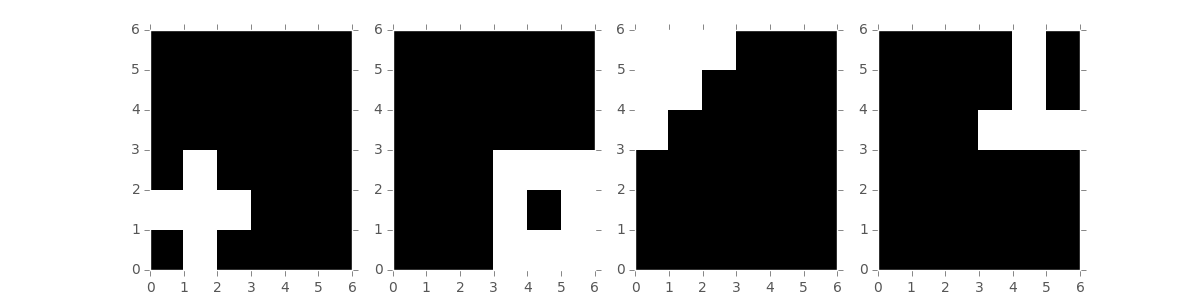
\includegraphics[width=\linewidth]{data_files/features.png}
\caption {Features/basis images used to simulate data}
\label{fig:feat}
\end{figure}

\begin{figure}
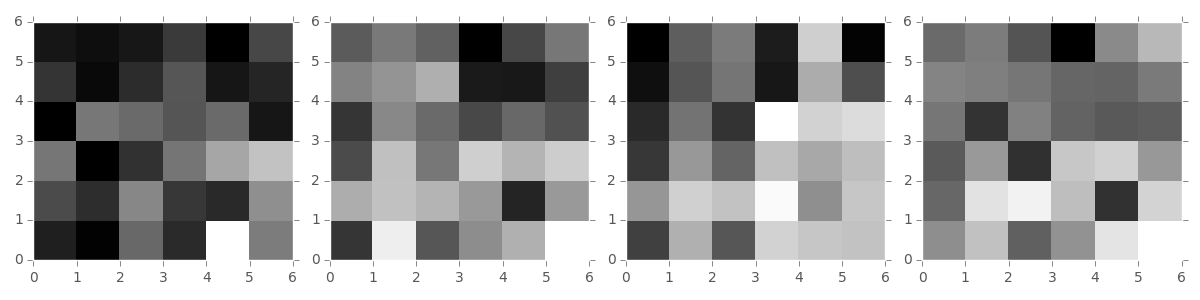
\includegraphics[width=\linewidth]{data_files/data.png}
\caption {Simulated data (first four of 100 images)}
\label{fig:dataaa}
\end{figure}

\subsection{Results}
We ran our code for 1000 iterations of the sampler to get convergence to the true values, for K, $\alpha$, $\sigma_{X}$ and $\sigma_{A}$ as can be seen in the trace plots in Figure \ref{fig:darr}.

\begin{figure}
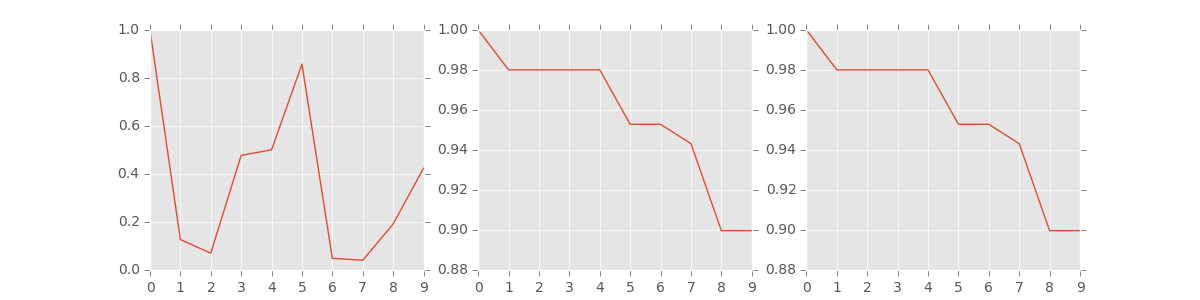
\includegraphics[width=\linewidth]{data_files/trace_plots.png}
\caption {Trace plots for K, alpha, sigma X and sigma A}
\label{fig:darr}
\end{figure}

\subsubsection{Detection of total number of latent features}
In Figure \ref{fig:figur} (a), we see that the mode of K is around six because the samples tended to include the four features used by a large number of images/objects and then a few features used by one one or two objects (which came in the form of added noise). Figure \ref{fig:figur} (b) shows the mean frequency with which objects tended to possess the features. We clearly see that most of the objects possessed only features 1, 2, 3 and 4. The extra features (5, 6 etc.) are possesed by very few objects which confirms that they are because of noise and not actual features.\\

We, thus, conclude the posterior mean of K to be 4, i.e. our code detected 4 latent features to be present in the data, which is as we would expect because we used 4 features to simulate the data in the beginning.

\begin{figure}
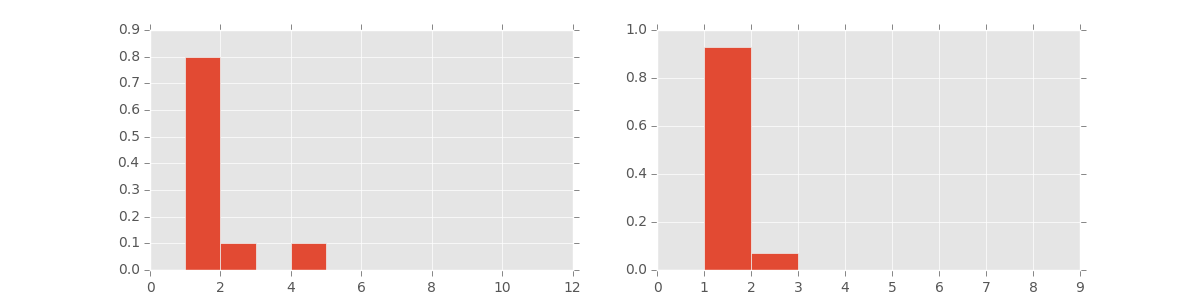
\includegraphics[width=\linewidth]{data_files/figures.png}
\caption {Histograms. (a) Posterior of K (b) Features (ordered by frequency of occurence)}
\label{fig:figur}
\end{figure}

\subsubsection{Detection of latent features present in each object and Object Reconstruction}
Figure \ref{fig:dat} shows the four most frequent features detected after the 1000 iterations of the sampler. We see that these features are the same as the features used to simulate the data as in Figure \ref{fig:feat}. They are just re-ordered.\\

Next, we recontruct the images using $X_{i} \sim N(Z_{i}A,0)$, where the posterior mean of the feature weights matrix A, given X and posterior means of Z, $\sigma_{A}$ and $\sigma_{X}$ is:
\[
E[A|X,Z] = (Z^TZ+\frac{\sigma_X^2}{\sigma_A^2}I)^{-1}Z^TX
\]
Figure \ref{fig:da} shows the posterior means of the reconstructions of the four original data images. The reconstructions provided by the model in Figure \ref{fig:da} clearly pick out the relevant features present in each image, despite the high level of noise as seen in Figure \ref{fig:dataaa}.\\

\begin{figure}
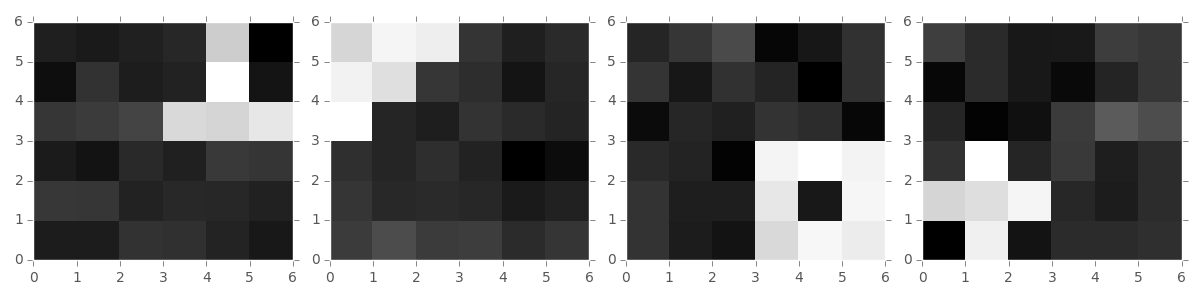
\includegraphics[width=\linewidth]{data_files/detected_features.png}
\caption {Features detected by code}
\label{fig:dat}
\end{figure}

\begin{figure}
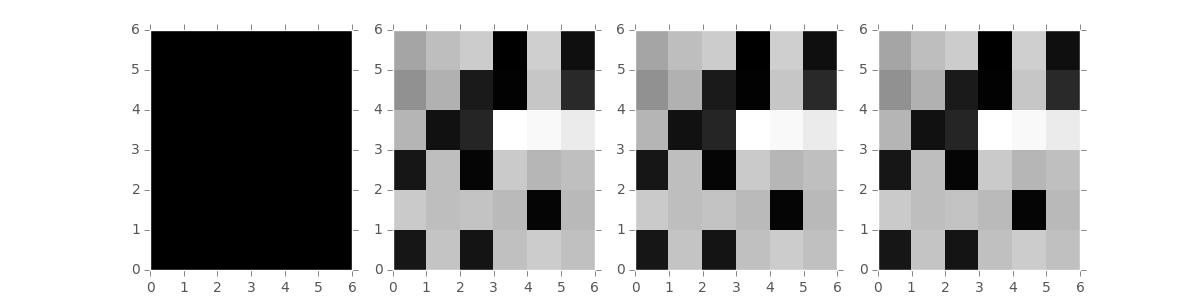
\includegraphics[width=\linewidth]{data_files/detected_total_features.png}
\caption {Reconstructed images}
\label{fig:da}
\end{figure}

\subsubsection{Validation}
To check the validity, Table \ref{featu} shows the features initially present (used to simulate) in the first four simulated images, where F1, F2, F3 and F4 refer to the order of features in Figure \ref{fig:feat}. We clearly see that the reconstructed images, as in Figure \ref{fig:da}, pick exactly the same features. The first reconstructed image (refer Figure \ref{fig:da}) picks feature 2, the 2nd picks 1 and 2, 3rd picks 1, 2 and 4 and 4th again picks 1 and 2 (feature numbering is as in Figure \ref{fig:feat}). This result shows that reconstructed images picked exactly the same features as were used to simulate them (Table \ref{featu}). This validates our model. 

\begin{table}[ht]
\centering
\caption{Presence/absence of latent features in the simulated data. 1 denotes presence, 0 denotes absence. F1, F2, F3, F4 refer to the 4 features in Figure \ref{fig:feat} (in that oreder) \label{featu}}
\begin{tabular}{lrrrr}
\toprule
{} &  F1 &  F2 &  F3 &  F4 \\
\midrule
1st image &   0 &   1 &   0 &   0 \\
2nd image &   1 &   1 &   0 &   0 \\
3rd image &   1 &   1 &   0 &   1 \\
4th image &   1 &   1 &   0 &   0 \\
\bottomrule
\end{tabular}

\end{table}

\section{Comparison}
We compare our algorithm with an implementation of the same algorithm in MATLAB. We also contrast our algorithm to another similar problem called Chinese Restaurant Process.

\subsection{Comparison with MATLAB implementation}
We compare our code and results to the MATLAB implementation of Indian Buffet Process provided by Yildirim [3]. The dataset he uses is the same as the one we have used. We got exactly similar results in terms of the features detected (Figure \ref{fig:dat}) and the reconstructed images (Figure \ref{fig:da}). We then profiled his MATLAB code and got results as shown in Figure \ref{fig:matlab}. We can see that the time taken for 1000 iterations of the sampler in MATLAB is 410 seconds which is significantly larger than the time taken by our most optimized version i.e. about 300 seconds (see Table \ref{time}). Therefore, even though we have a lot of matrix calculations and MATLAB is the suited platform to run matrix intensive codes, we are able to write a much more efficient code in Python.

\begin{figure}
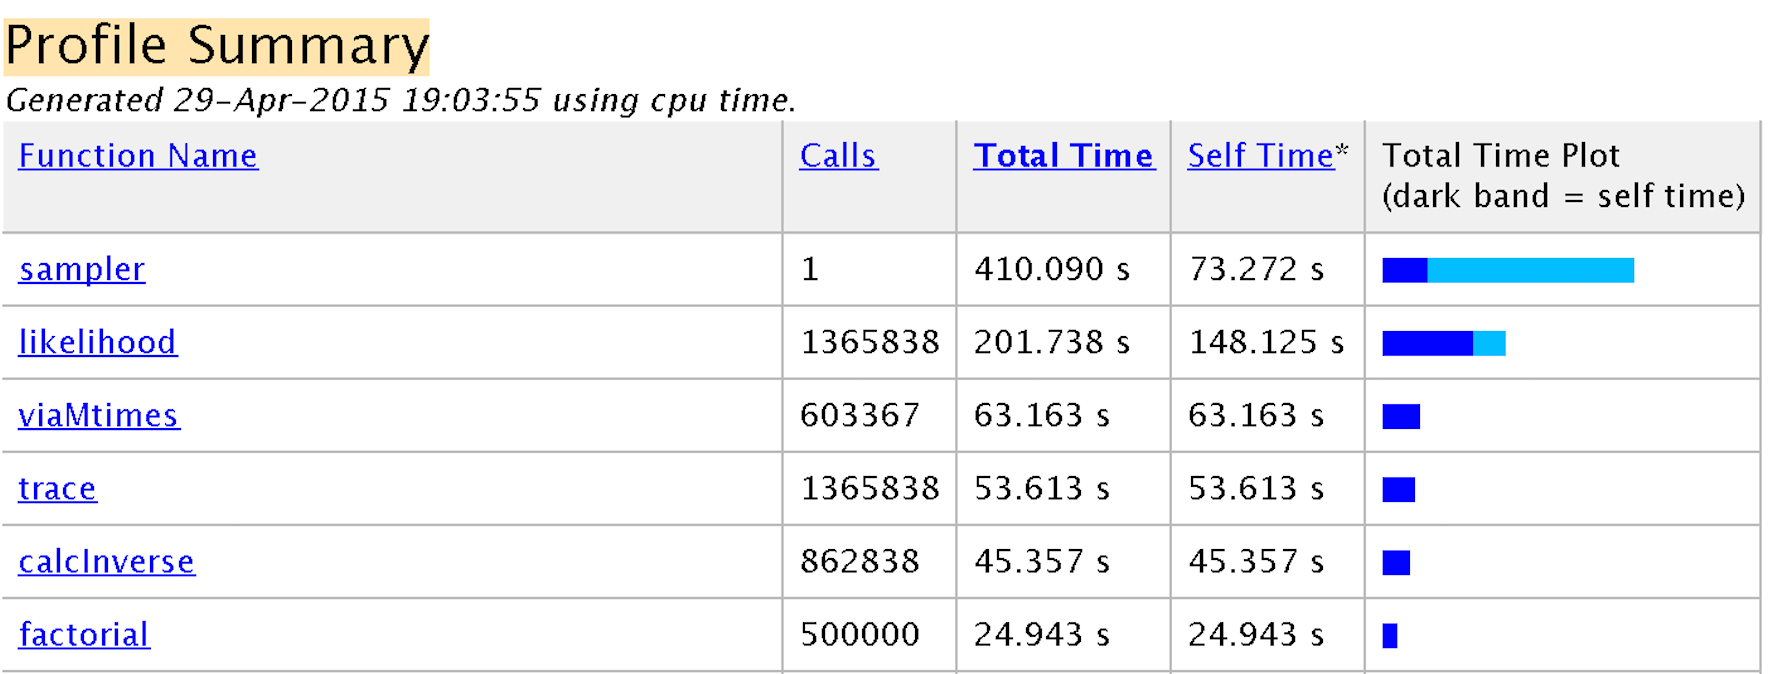
\includegraphics[width=\linewidth]{matlab_profile.png}
\caption {Profiling results of matlab code for IBP}
\label{fig:matlab}
\end{figure}

\subsection{Comparison with Chinese Restaurant Process}
Chinese Restaurant Process is an algorithm of customers’ seating in a Chinese Restaurant with infinite tables and infinite seats in each table. The customers enter one after the other and choose a table at random. In the CRP with parameter $\alpha$, each customer chooses an occupied table with probability proportional to the number of occupants and chooses the next vacant table with probability $\alpha$.\\

Both IBP and CRP model latent features and allow for infinite features but solve slightly different problems. CRP solves the clustering problem and IBP solves feature allocation problem. IBP allows each customer to be assigned to multiple features (dishes), while
CRP assigns each customer to a single feature (table). Figures \ref{fig:IBP} and \ref{fig:CRP}, from Gershman and Blei (2012) [4], diagramatically portray the difference between the two processes. Clearly, IBP solves a much wider problem in that it allows an object to have multiple features.

\begin{figure}
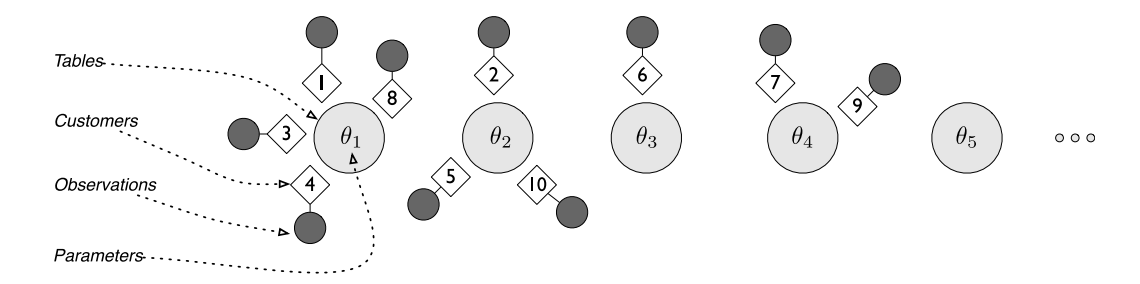
\includegraphics[width=\linewidth]{IBP.png}
\caption {Indian Buffet Process}
\label{fig:IBP}
\end{figure}

\begin{figure}
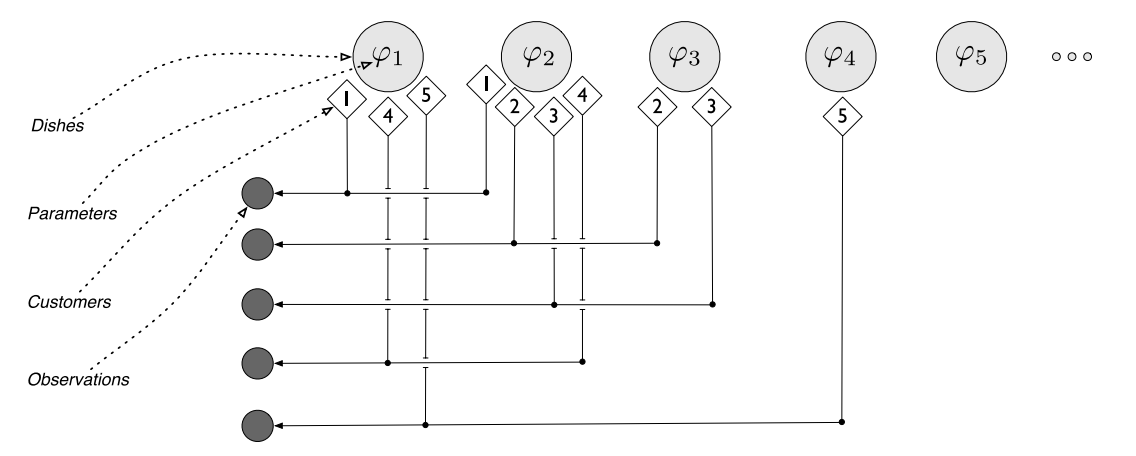
\includegraphics[width=\linewidth]{CRP.png}
\caption {Chinese Restaurant Process}
\label{fig:CRP}
\end{figure}

\newpage
\section{Conclusion}
We derived and tested an Infinite Linear-Gaussian Binary Latent Feature model, using IBP as the prior, to detect the underlying features in a noisy image dataset. We validated our results by detecting the same features that were used to simulate the images. The basic code was written in Python, which was then optimized by removing redundant calculations and code statements and vectorization. Cython, JIT and high performance computing tools were tested. Since the code is highly dependent on matrix calculations and our profiling showed that approximate matrix inversion proposed by Griffiths and Ghahramani [1] was faster than full rank matrix inverse, future work would involve obtaining a stable Markov Chain with this approximate inverse technique.

\begin{thebibliography}{9}

\bibitem{lampor}
  Thomas Griffiths and Zoubin Ghahramani,
  \emph{Infinite Latent Feature Models and the Indian Buffet Process},
  Technical report, Gatsby Computational Neuroscience Unit, 
  2005.
  
\bibitem{lampo94}
  Thomas Griffiths and Zoubin Ghahramani,
  \emph{Infinite Latent Feature Models and the Indian Buffet Process},
  In Advances in Neural Information Processing Systems, volume 18. NIPS Proceedings,
  2005.
  
\bibitem{lampor94}
  Ilker Yildirim,
  \emph{Bayesian Statistics: Indian Buffet Process}, homepage link (with sample code): http://www.mit.edu/~ilkery/
  
\bibitem{lampore}
  Samuel J Gershman and David M Blei,
  \emph{A Tutorial on Bayesian Nonparametric Models},
  Journal of Mathematical Psychology, 
  2012.
  
\bibitem{lamprror}
  Ilker Yildirim and Robert A Jacobs,
  \emph{A Bayesian Nonparametric Approach to Multisensory Perception},
  The Cognitive Science society, 
  2010.
  
\end{thebibliography}




\end{document}